\section{Theory}
\label{sec:theorie}
This part of the lab protocol will discuss the theory behind the heat capacity of condensed matter.
The different models of heat capacity will be shown and their motivation and usage will be described.
\subsection{Classical model}
Heat capacity 
\begin{equation}
    C = \frac{\Delta Q}{\Delta T}
    \label{eq:heat_capacity}
\end{equation}
is described as the amount of heat energy $\Delta Q$ that is needed to heat a probe by the temperature $\Delta T$.
With the first law of thermodynamics, it is then possible to describe the amount of heat $\Delta Q$ in a more accurate way.
The first law of thermodynamics states 
\begin{equation*}
    \symup{d}Q = \symup{d}U + p\symup{V}
\end{equation*}
the infinitesimal amount of heat $\symup{d}Q$ equals the inner energy $\symup{d}U$ added by the work done by the system or on the system.
Now two different heat capacities derive from the equation \eqref{eq:heat_capacity} depending on the circumstances.
If the probe is heated up while its volume stays the same $\symup{d}V=0$ the heat capacity will be 
\begin{equation}
    C_\text{V} = \frac{\symup{d}U}{\symup{d}T}
    \label{eq:heat_cap_v}
\end{equation}
which is easy to calculate, but hard to measure.
If the probe is heated up by constant pressure the calculations will be hard but it is easier to measure the heat capacity as the heat expansion or contraction does not matter.
To calculate the heat capacity at constant pressure $c_\text{p}$ from the heat capacity of a constant volume $c_\text{v}$ the formula
\begin{equation}
    c_\text{p} - c_\text{v} = TVB\alpha_\text{V}^2
    \label{eq:correction_formula}
\end{equation}
can be used.
It contains the bulk module 
\begin{equation*}
\frac{1}{B} = - \frac{1}{V} \left (\frac{\partial  V}{\partial p} \right )_T
\end{equation*}
and the kompression module
\begin{equation*}
    \alpha_v = \frac{1}{V} \left( \frac{\partial V}{\partial T}\right )_p\, .
\end{equation*}
\subsection{Dulong-Petit}
As already mentioned the easiest way to calculate the heat capacity of a probe is to assume a constant volume.
By doing so just the inner energy needs to be derived by the temperature $T$.
In the classical model the inner energy
\begin{equation*}
    U = \frac{f}{2}Nk_\text{B}T
\end{equation*}
with $f$ being the degrees of freedom, $N$ the number of atoms, $k_\text{B}$ the Boltzman constant and $T$ the temperature.
The classical model assumes that the heat capacity is given by the amount of oscillating atmos $N$ inside the probe.
Because the atoms can oscillate into three directions, they have $f=6$ degrees of freedom.
This means the heat capacity at constant volume can be written as 
\begin{equation*}
    c_\text{v} = \frac{\symup{d}U}{\symup{d}T} = 3Nk_\text{B}
\end{equation*}
which further simplifies to the law of Dulong-Petit
\begin{equation}
    c_\text{v,mol} = 3R
    \label{eq:dulong}
\end{equation}
if we plug in the Avogardo constant $N_\text{A} = N$ for the number of atoms and write $R = N_\text{A} k_\text{B}$, with $R$ being the gas constant.
The law of Dulong-Petit is a good approximation for some metals at high temperatures above $T = \SI{300}{\K}$.
However, it loses its accuracy for lower temperature at which the influence of quantum effects can not be neglected anymore.
\subsection{Einstein model}
As already mentioned the classical model breaks apart at low temperatures.
This is due to the impossibility of lattice oscillations, which are called phonons, to take any energy level.
Similar to the harmonic oscillator, phonons can just take on discrete energy
\begin{equation*}
    E_n = (n +\frac{1}{2})\hbar\omega
\end{equation*}
with $n$ being a natural number called the occupation number, $\omega$ being its eigenfrequency and $\hbar$ being the reduced Planck constant.
As their energy $\hbar\omega>>k_\text{B}T$ becomes bigger than the energy given by the temperature they can not promote to a different energy level.
This behavior is illustrated in figure \ref{fig:energy_phonon}.
\begin{figure}
    \centering
    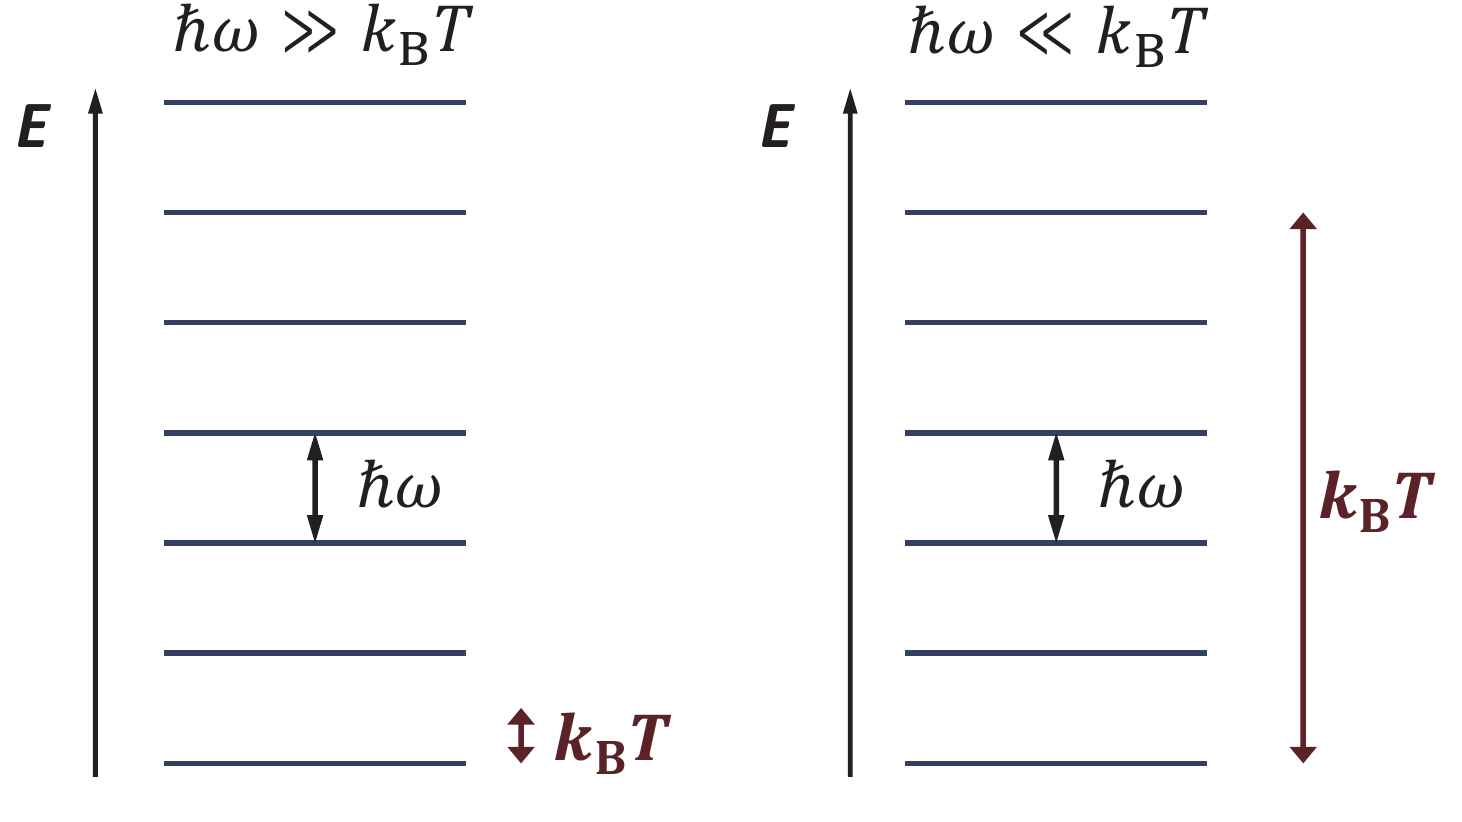
\includegraphics[width=0.6\textwidth]{content/pictures/energy.png}
    \caption{The picture illustrates the impossibility of a phonon to absorb heat energy as the temperature lowers beneath the possible energy that the phonon can take on.}
    \label{fig:energy_phonon}
\end{figure}
Because of the quantized nature of phonon energy the average inner energy $<U>$ becomes
\begin{equation}
    <U> = U_\text{eq} + 3N\hbar\omega(\frac{1}{2} + <n>)
    \label{eq:inner_energy}
\end{equation}
where $U_\text{eq}$ is the inner energy in equilibrium.
One model that takes the quantum effects into account is the Einstein model.
In this model, all the phonon modes are given the same possible eigenfrequency $\omega_\text{E}$.
This assumption suits optical phonons, acoustic phonons however, do not show this behavior. 
With this assumption the average inner energy 
\begin{equation*}
    <U> = 3N\hbar\omega_\text{E} \left ( \frac{1}{2} + \frac{1}{\symup{e}^{\hbar\omega_\text{E}/k_\text{B}T} - 1}\right )
\end{equation*}
can be calculated by equation \eqref{eq:inner_energy}.
The heat capacity in the Einstein model is now calculate by equation \eqref{eq:heat_cap_v}.
The substitution 
\begin{equation*}
    \Theta_\text{E} = \frac{\hbar\omega_\text{E}}{k_\text{B}}
\end{equation*}
finally gives the heat capacity at constant volume
\begin{equation*}
    c_v ^{\text{E}} = 3 N k_\text{B} \left ( \frac{\Theta_\text{E}}{T} \right )^2 \frac{ \symup{e}^{\Theta_\text{E}/T}}{\left [ \symup{e}^{\Theta_\text{E}/T} - 1 \right ]^2}
    \label{eq:heat_einstein}
\end{equation*}
in the Einstein model.
At low temperatures $T<<\Theta_\text{E}$ the heat capacity becomes 
\begin{equation*}
    c_v ^{\text{E}} = 3Nk_\text{B} \left ( \frac{\Theta_\text{E}}{T} \right )^2 \symup{e}^{-\Theta_\text{E}/T}
\end{equation*}
this result however, does not fit to measurements at low temperatures.
Experiments show that the heat capacity should have a $T^3$ depends at low temperatures.
The reason is that the einstein model does not model acoustic phonons, which are the main actors for heat capacity in condensed matter.
For this, a new model is needed.
\subsection{Debye model}
The Debye model makes the following assumptions.
First of all the possible phonon modes follow a linear dispersion as so 
\begin{equation*}
    \omega_\text{i} = v_\text{i} q
\end{equation*}
with $v_\text{i}$ being the velocity of sound in the medium and $q$ being the absolute value of the wave vector $\vec{q}$.
It should be mentioned that this assumption fits well for the dispersion behavior of acoustic phonons.
Secondly the sum over all wave vectors $\vec{q}$ in the first Brillouin-Zone becomes an integral over a sphere with the same volume as the first Brillouin-Zone.
The radius of this sphere is the Debye-wavevector 
\begin{equation*}
    q_D = \left ( 6 \pi^2 \frac{N}{V} \right )^{1/3}
\end{equation*}
with which the debye temperature
\begin{equation*}
    \Theta_\text{D} = \frac{\hbar v_s q_{D}}{k_\text{B}}
\end{equation*}
can be defined.
With one more substitution $x :=  \hbar v_s q / k_\text{B}T$ the heat capacity in the Debye model can be expressed as
\begin{equation*}
    c_v ^{\text{D}} = 9 N k_\text{B} \left (\frac{T}{\Theta_\text{D}} \right )^3 \int_0^{\Theta_\text{D}/T} \frac{x^4 \symup{e}^x \symup{d}x}{\left( \symup{e}^x - 1\right)^2} \, .
    \label{eq:heat_debye}
\end{equation*}
As the goal is to find a good approximation of the heat capacity at lower temperature the heat capacity for temperature $T<<\Theta_\text{D}$ is looked at.
The result is the exprenssion
\begin{equation*}
    c_v ^{\text{D}} = \frac{12 \pi^4}{5} N k_\text{B} \left ( \frac{T}{\Theta_\text{D}} \right )^3
\end{equation*}
which shows the desired $T^3$ depends at lower temperatures.\\\\
The difference in the behavior at lower temperatures between the Einstein model and the Debye model can be seen in figure \ref{fig:ein_deb}.
Moreover, the $T^3$ and $\symup{e}^{-T}$ are well distinguishable as the exponential falls to zero way faster.
\begin{figure}
    \centering
    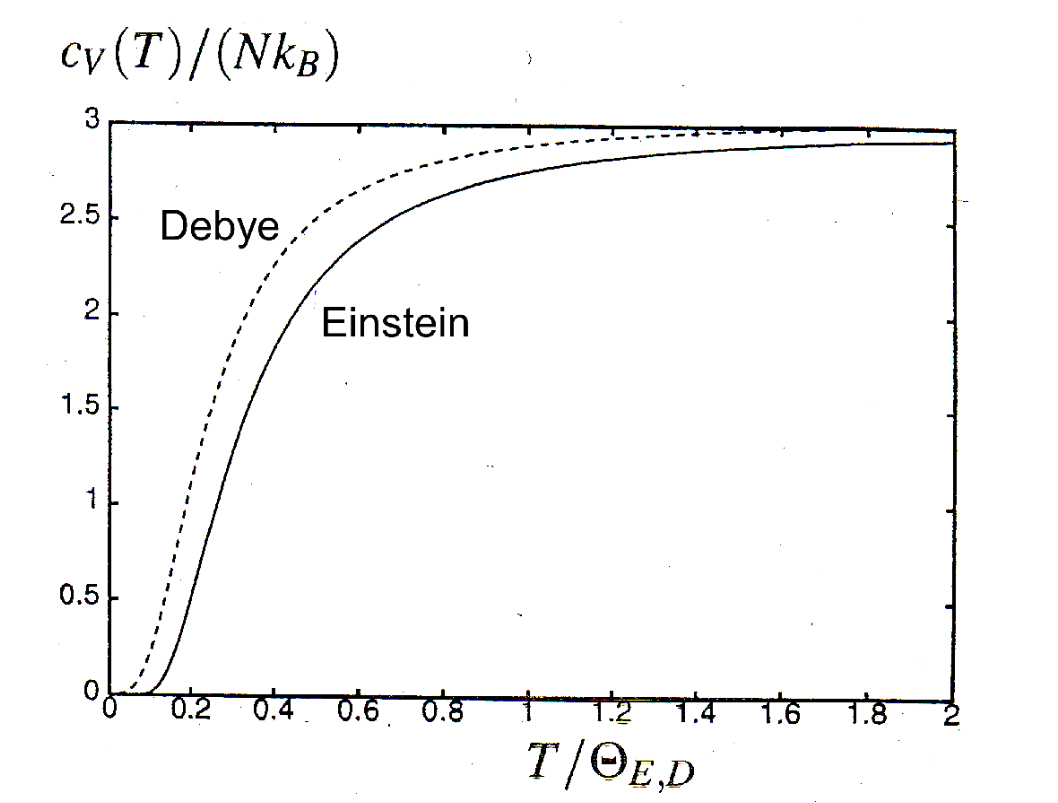
\includegraphics[width=0.5\textwidth]{content/pictures/debye_ein.png}
    \caption{The heat capacity in the Einstein and the Debye model is plotted against the temperature. As the Einstein model contains a $\symup{e}^{-T}$ depends in temperature it falls way faster.}
    \label{fig:ein_deb}
\end{figure}